\section{Vorbereitung}
Vor der Durchführung eines Penetrationstests müssen verschiedenste Aufgaben erledigt und Rahmenbedingungen geklärt werden.

\subsection{Aufwandsschätzung}
	Ein äußert wichtiger aber auch sehr schwieriger Punkt ist die Aufwandsschätzung. Natürlich können klassische Methoden der Aufwandsschätzung aus dem Bereich der Projektmanagement verwendet werden, jedoch müssen eine Vielzahl weitere technischer Aspekte betrachtet werden.\\
	
	Viele Firmen berechnen den Aufwand aus der Anzahl der Eingabefelder. Leider ist diese Vorgehensweise oft nicht zielführend, da die Komplexität des dahinter liegenden Systems nicht in Betracht gezogen wird. Wird zum Beispiel eine Webseite mit einem Framework erstellt, welches Eingaben stetig Filtert, ist die Wahrscheinlichkeit eine XSS oder SQLi zu finden unabhängig von der Anzahl der Eingabefelder gering. In diesem Fall sollte man andere Komponenten wie die Authentisierungslogik oder den Webserver selbst angreifen. Dies würde durch die Aufwandsschätzung rein nach Eingabefeldern nicht in Betracht gezogen. Eine weitere Möglichkeit wäre die Einschätzung anhand der Anzahl der zu testenden IP-Adressen. Leider gibt es hier ähnliche Probleme wie bei der Anzahl der Eingabefelder, da auch hier nicht die Komplexität der Anwendung an sich mit einbezogen wird.\\

Insgesamt müssen viele Teilaspekte beachtet werden, damit die Pentester ein Gefühl für die Anwendung bekommen und den groben Aufwand schätzen können. Um dies zu vereinfachen, wurden im ersten Schritt Fragen erarbeitet. Als Grundlage hierfür dienten die Fragen von \url{http://www.pentest-standard.org/index.php/Pre-engagement}. Zusätzlich wurden Fragen und Kategorien ergänzt, welche sich während der Tätigkeit des Autors bei der Allianz Deutschland AG als hilfreich oder notwendig erwiesen haben. Die Kategorien und Fragen sind in der Sektion \ref{ref:KategorienUndFragen} dargestellt.\\

Anschließend galt es, die Fragen in eine passende Form zu bringen. Dazu wurden im ersten Versuch ein LaTeX-Dokument erstellt. Dies ist in Sektion \ref{ref:AufImplInTex} dargestellt. Trotz der Ansprechenden Form sind LaTeX-Dokumente meistens nicht sehr intuitiv und effizient auszufüllen. Daher wurde eine Webanwendung implementiert, welche den Aufwandsfragebogen darstellt und ein einfaches Ausfüllen ermöglicht. Dies Technik und Vorgehensweise ist in Sektion \ref{ref:AufImplInWeb} dargestellt.

TODO Docker

\subsubsection{Fragebogen}\label{ref:KategorienUndFragen}
Um einen groben Eindruck vom Umfang des Tests zu bekommen, empfiehlt sich die Durchsprache eines standardisierten Fragebogens. Im Rahmen dieser Arbeit wurde der Fragebogen von Pentest-Standard.org TODO(Link) übersetzt und erweitert. Anschließend wurde der Fragebogen mit der Ansprechpartnern der Allianz Deutschland AG diskutiert und ergänzt, sodass sich folgende Fragen ergeben:

\paragraph{Allgemein}
\begin{itemize}
	\item Wie ist der Projekt-Name?
	\item Wer sind die Ansprechpartner?
	\item Welche Art/en von Pentest/s sollen durchgeführt werden? \\
	(Web-Application/Web-Service/Mobile-Application/Network/Social Engineering/Wireless/Physical)
	\item Ist der Test für eine spezielle Compliance-Anforderung notwendig?\\
	(Ja/Nein)
	\item Wann soll der Test durchgeführt werden?
	\item In welchen Zeiträumen soll der Test durchgeführt werden?\\
	(Bürozeiten/Feierabend/Wochenende)
\end{itemize}

\paragraph{Web Application Penetration Test}
\begin{itemize}
	\item Wie geschieht der Zugriff auf die Anwendung?\\
	(Aus dem Internet erreichbar/IP-Einschränkung/VPN/Pentest muss intern durchgeführt werden)
	\item Welche Funktionalitäten hat die Anwendung?\\
	(CMS/Captcha/Upload/Download/Browser-Plugins/Workflows)
	\item In welcher Stage befindet sich die Anwendung?\\
	(Development oder Test/System Integration/Produktion)
	\item Wird der Quellcode der Applikation/Webseite zugänglich gemacht?\\
	(Ja/Nein)
	\item Wie viele Web-Applikationen sind In-Scope?
	\item Wie viele Login-Systeme sind In-Scope?
	\item Wie viele statische Seiten sind ca. In-Scope?
	\item Wie viele dynamische Seiten sind ca. In-Scope?
	\item Soll Fuzzing gegen die Applikation/en eingesetzt werden?\\
	(Ja/Nein)
	\item Soll der Penetrations-Test aus verschiedenen Rollen durchgeführt werden?\\
	(Ja/Nein)
	\item  Wie ist die Anmeldung gestaltet?\\
	(Benutzername und Passwort/Zertifikat/Komplexeres System)
	\item Welche Technologien nutzt die Anwendung?
	\item Sollen Password-Scans auf die Webseite durchgeführt werden?\\
	(Ja/Nein)
\end{itemize}

\paragraph{Web Service Penetration Test}
\begin{itemize}
	\item Wie geschieht der Zugriff auf die Anwendung?\\
	(Aus dem Internet erreichbar/IP-Einschränkung/VPN/Pentest muss intern durchgeführt werden)
	\item In welcher Stage befindet sich die Anwendung?\\
	(Development oder Test/System Integration/Produktion)
	\item Wird der Quellcode des Services zugänglich gemacht? \\
	(Ja/Nein)
	\item Wie viele Web-Services sind In-Scope?
	\item Soll Fuzzing gegen die Applikation/en eingesetzt werden?\\
	(Ja/Nein)
	\item Soll der Penetrations-Test aus verschiedenen Rollen durchgeführt werden?\\
	(Ja/Nein)
	\item  Wie ist die Anmeldung gestaltet?\\
	(Benutzername und Passwort/Zertifikat/Komplexeres System)
	\item Welche Technologien wurden für den Service genutzt??
	\item Sollen Password-Scans auf die Webseite durchgeführt werden?\\
	(Ja/Nein)
\end{itemize}

\paragraph{Mobile Application Penetration Test}
\begin{itemize}
	\item Welche Technologien wurden für die App genutzt?
	\item Wird der Quellcode der App zugänglich gemacht?\\
	(Ja/Nein)
	\item Gibt es eine Root-Detection? Wenn ja, welche Konsequenzen hat eine postive Erkennung?\\
	(Ja/Nein)
	\item Hat die App einen Login?\\
	(Ja/Nein)
	\item Soll der Penetrations-Test aus verschiedenen Rollen durchgeführt werden?\\
	(Ja/Nein)
	\item Soll Fuzzing gegen die App eingesetzt werden?\\
	(Ja/Nein)
\end{itemize}

\paragraph{Network Penetration Test}
\begin{itemize}
	\item Was ist das Ziel des Penetrations-Test?
	\item Wie viele IP-Adressen sollen getestet werden?
	\item Sind Techniken im Einsatz, die die Resultate verfälschen könnten? (WAF, IPS etc.?)\\
	(Ja/Nein)
	\item Wie ist das Vorgehen bei einem gelungenen Angriff?
	\item Soll versucht werden lokale Admin-Rechte zu erlangen und tiefer in das Netz vorzudringen?\\
	(Ja/Nein)
	\item Sollen Angriffe auf gefundene Passwort-Hashes durchgeführt werden?\\
	(Ja/Nein)
\end{itemize}

\paragraph{Social Engineering}
\begin{itemize}
	\item Gibt es eine vollständige Liste von E-Mail-Adressen, die für den Test verwendet werden können?\\
	(Ja/Nein)
	\item Gibt es eine vollständige Liste von Telefon-Nummern, die für den Test verwendet werden können?\\
	(Ja/Nein)
	\item Ist das Einsetzen von Social Engineering zum Überwinden physikalischer Sicherheitseinrichtungen erlaubt?\\
	(Ja/Nein)
	\item Wie viele Personen sollen ca. getestet werden?
\end{itemize}

\paragraph{Wireless Network Penetration Test}
\begin{itemize}
	\item Wie viele Funk-Netzwerke sind im Einsatz?
	\item Gibt es eine Gäste WLAN? Wenn ja, wie ist dieses Umgesetzt?\\
	(Ja/Nein)
	\item Welche Verschlüsselung wird für die Netzwerke genutzt?
	\item Sollen nicht-firmen-Geräte im WLAN aufgespürt werden?\\
	(Ja/Nein)
	\item Sollen Netz-Attacken gegen Clients durchgeführt werden?\\
	(Ja/Nein)
	\item Wie viele Clients nutzen das WLAN ca.?
\end{itemize}

\paragraph{Physical Penetration Test}
\begin{itemize}
	\item Wie viele Einrichtungen sollen getestet werden?
	\item Wird die Einrichtung mit anderen Parteien geteilt?\\
	(Ja/Nein)
	\item Muss Sicherheitspersonal umgangen werden?\\
	(Ja/Nein)
	\item Wird das Sicherheitspersonal durch einen Dritten gestellt?\\
	(Ja/Nein)
	\item Ist das Sicherheitspersonal bewaffnet?\\
	(Ja/Nein)
	\item Ist der Einsatz von körperlicher Gewalt durch das Sicherheitspersonal gestattet?\\
	(Ja/Nein)
	\item Wie viele Eingänge gibt es zu der/den Einrichtung/en?
	\item Ist das knacken von Schlössern oder fälschen von Schlüsseln erlaubt?\\
	(Ja/Nein)
	\item Wie groß ist die Fläche ungefähr?
	\item Sind alle physikalischen Sicherheitsmaßnahmen dokumentiert und werden zur Verfügung gestellt?\\
	(Ja/Nein)
	\item Werden Video-Kameras verwendet?\\
	(Ja/Nein)
	\item Werden diese Kameras durch Dritte verwaltet?\\
	(Ja/Nein)
	\item Soll versucht werden, die aufgezeichneten Daten zu löschen?\\
	(Ja/Nein)
	\item Gibt es ein Alarm-System?\\
	(Ja/Nein)
	\item Gibt es einen Stillen Alarm?\\
	(Ja/Nein)
	\item Welche Ereignisse lösen den Alarm aus?
\end{itemize}

\paragraph{Fragen an den System-Administrator}
\begin{itemize}
	\item Gibt es Systeme, die als instabil angesehen werden (alte Patch-Stände, Legacy Systeme etc.)?\\
	(Ja/Nein)
	\item Gibt es Systeme von Dritten, die ausgeschlossen werden müssen oder für die weitere Genehmigungen notwendig sind?\\
	(Ja/Nein)
	\item Was ist die Durchschnittszeit zur Wiederherstellung der Funktionalität eines Services?
	\item Ist eine Monitoring-Software im Einsatz?\\
	(Ja/Nein)
	\item Welche sind die kritischsten Applikationen?
	\item Werden in einem regelmäßigen Turnus Backups erstellt und getestet?\\
	(Ja/Nein)
	\item Fragen an den Business Unit Manager
	\item Ist die Führungsebene über den Test informiert?\\
	(Ja/Nein)
	\item Welche Daten stellen das größte Risiko dar, falls diese manipuliert werden?
	\item Gibt es Testfälle, die die Funktionalität der Services prüfen und belegen können?\\
	(Ja/Nein)
	\item Sind "Disaster Recovery Procedures" vorhanden?\\
	(Ja/Nein)
\end{itemize}

Dabei müssen natürlich nur die für die Art des Pentests (Web-Application/Network/Social Engineering/Wireless/Physical) durchgeführt werden.

\subsubsection{Implementierung in Latex}\label{ref:AufImplInTex}
Nachdem der Festlegung der Fragen, wurde der Fragebogen in LaTeX implementiert. Dabei wurde speziell das Format angepasst, sodass eine ausgedruckte Kopie des Fragebogens möglichst effizent ausgefüllt werden kann. Dafür wurden die Fragen in Boxen integriert, sowie Ja/Nein-Antworten ansprechend dargestellt. Die angepasste Formatierung ist in Abbildung \ref{fig:FragLatex} dargestellt.\\

\begin{figure}[htbp]
	\centering
	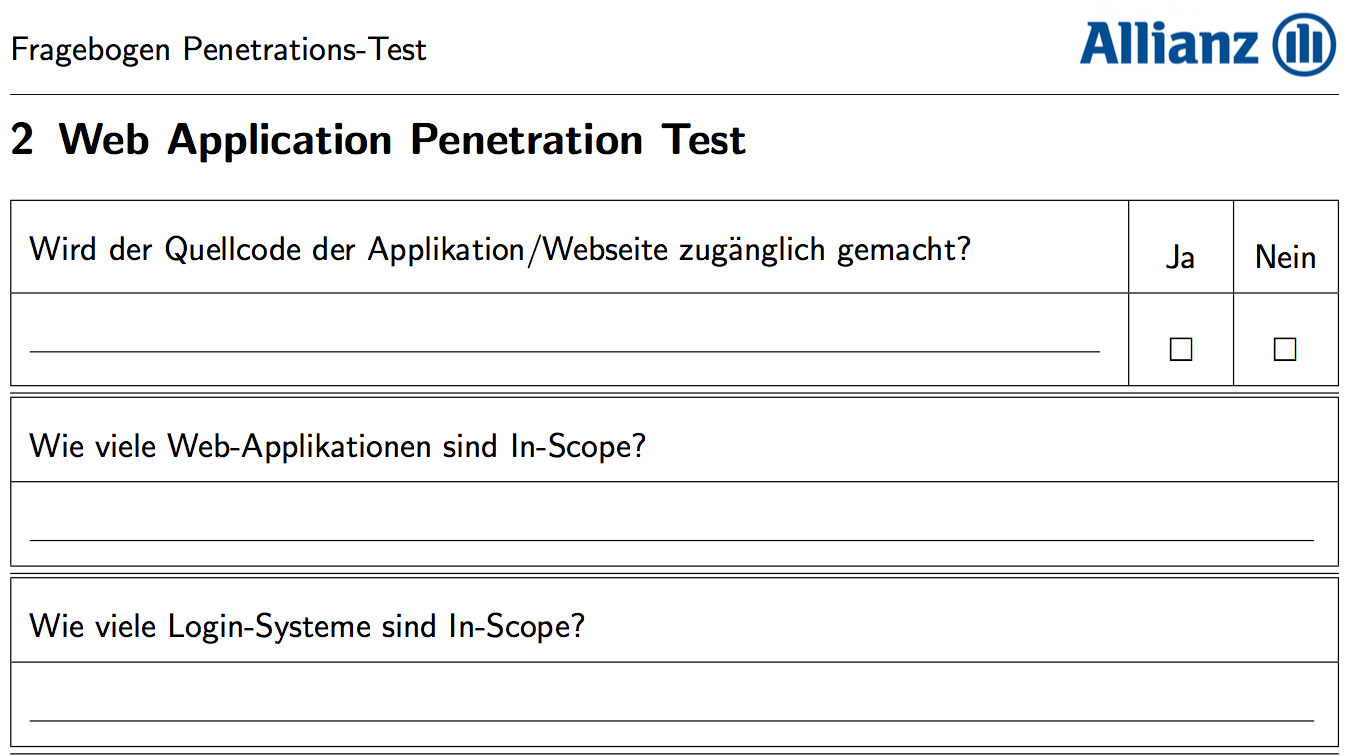
\includegraphics[width=\textwidth]{bilder/pentest_prozesse/vorbereitung/fragebogen_latex.png}
	\caption{Ein kurzer Ausschnitt des Fragebogens mit formatierten Fragen}
	\label{fig:FragLatex}
\end{figure}

Um eine möglichst einfache Erweiterung der Fragen in LaTeX zu gewährleisten, wurden LaTeX-Makros für die jeweiligen Frage-Arten entworfen. Im Folgenden ist ein kurzes Beispiel für ein solches Makro und zwei Fragen, die dieses nutzen:

\lstset{language=Tex}
\begin{lstlisting}
\newcommand{\frageJaNein}[1]{\makebox[\textwidth]{%
\renewcommand{\arraystretch}{2.0}
\begin{tabularx}{\textwidth}{|X|S|S|}
  \hline
  #1 & Ja & Nein\\
  \hline
  \line(1,0){350} & $\square$ & $\square$	\\
  \hline \hline
\end{tabularx}%
\renewcommand{\arraystretch}{1.0}
}}

\frageJaNein{Soll der Penetrations-Test aus verschiedenen Rollen durchgeführt werden?}
\frageJaNein{Sollen Angriffe auf gefundene Passwort-Hashes durchgeführt werden?}
\end{lstlisting}

\subsubsection{Implementierung als Webabwendung}\label{ref:AufImplInWeb}
Die LaTeX-Implementierung ist gut geeignet, um den Fragebogen bei einem physikalischen Termin zu besprechen. Für ein Ausfüllen am Computer ist es jedoch weniger geeignet, da man mit einem passenden PDF-Reader die Antworten einfügen müsste. Daher wurde eine Webanwendung entworfen, welche das Ausfüllen am Computer, zum Beispiel parallel zu einem Online-Meeting, vereinfacht.\\

Um die Anwendung möglichst minimalistisch und einfach zu halten, wurde Python als Programmiersprache und Flask Web-Server verwendet. Auf HTML-Seite wurde Bootstrap 4 zur einfachen Formatierung genutzt.\\

Das Einfügen der Eingaben in der Weboberfläche wurde anfangs über eine einfache String-Substitution gelöst:
\lstset{language=Python}
\begin{lstlisting}
# Load template from file
orig_file = open(tex_path + "/Fragen.tex", 'r')
template = LaTeXTemplate(orig_file.read())
orig_file.close()

# Substitute with form-fields
new_string = template.substitute(
    allg_anspr_web_app=__html_to_tex(
        request.form['allg_anspr_web_app']
    ),
    allg_pen_art_wapt=__html_to_checkbox(
        request, 'allg_pen_art_wapt'
    ),
    # Andere Form-Felder
)
\end{lstlisting}

Da dies jedoch einen erhöhten Wartungsaufwand bei zum Beispiel Änderung von Parametern mit sich zieht, wurde die Substitution durch eine einfachere Implementierung in Jinja2 ersetzt. Die Substitutions-Technik von Jinja ist unter \ref{jinja2} aufgezeigt. Unter der Nutzung von Jinja-Makros können so sehr effizient die HTML-Dateien für die Fragen erstellt werden. Im Folgenden ist ein kurzes Beispiel aus dem Fragebogen bezüglich Web-Application Penetration Tests, in welchem einige Fragen definiert werden:
\begin{lstlisting}
{{ binary_question("wapt_quell_zug", "Wird der Quellcode der Applikation/Webseite zugänglich gemacht?") }}
  {{ text_question("wapt_anz_web_app", "Wie viele Web-Applikationen sind In-Scope?") }}
  {{ text_question("wapt_anz_login_sys", "Wie viele Login-Systeme sind In-Scope?") }}
\end{lstlisting} 

Durch die Verwendung von Bootstrap ist die Anwendung automatisch "`responsive"', also unter verschiedenen Auflösungen verwendbar. Ein Screenshot der Anwendung ist unter \ref{fig:FragWeb} dargestellt.

\begin{figure}[htbp]
	\centering
	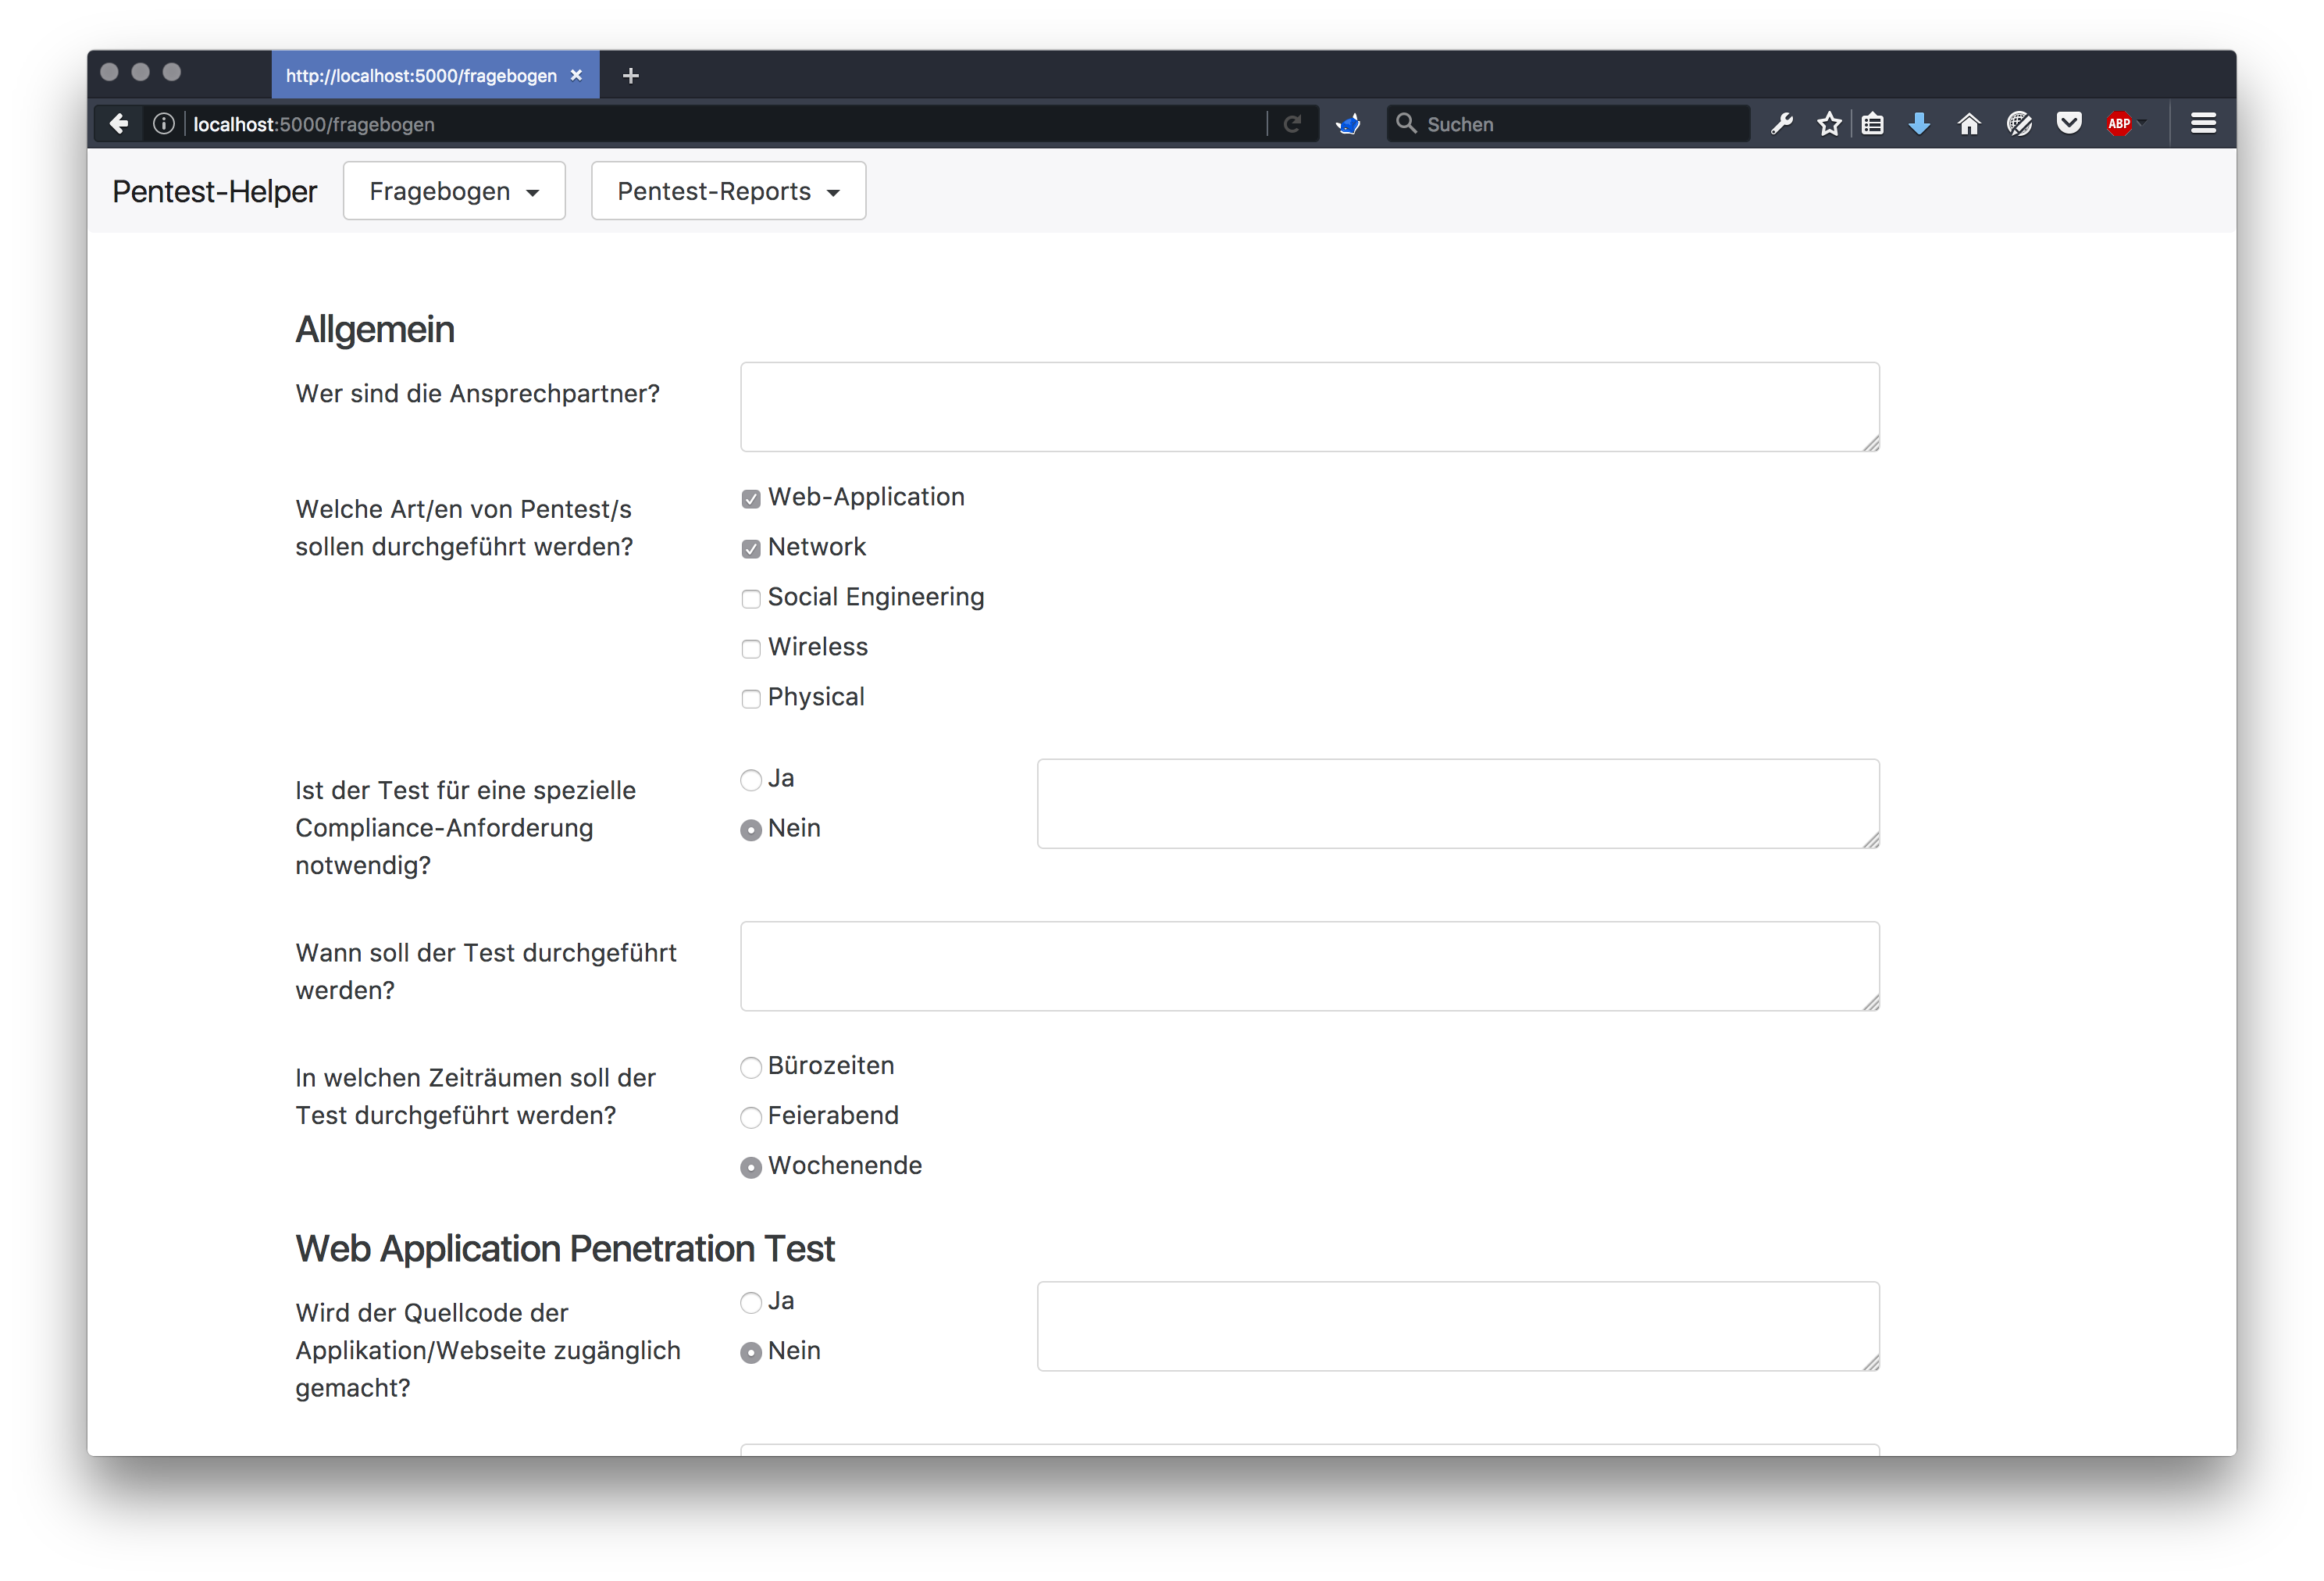
\includegraphics[width=\textwidth]{bilder/pentest_prozesse/vorbereitung/fragebogen_web.png}
	\caption{Ein kurzer Ausschnitt der Fragebogen-Webanwendung}
	\label{fig:FragWeb}
\end{figure}

Um die Daten dauerhaft zu speichern, wurde eine Datenbankanbindung implementiert. Hierzu wurde SQLAlchemy als Engine genutzt, da diese sehr gut zu Flask passt und sich einfach und ohne viel Aufwand implementieren lässt. Mehr zu SQLAlchemy ist de Abschnitt \ref{ref:SQLAlchemy} zu entnehmen.\\

Zum Erstellen des PDFs muss das generierte TeX-Dokument über \textit{pdflatex} umgewandelt werden. Dies geschieht im Quellcode folgendermaßen:
\begin{lstlisting}
try:
    # Double-Compile for ToC and refs
    subprocess.check_output(
        [
            '/usr/local/texlive/2016/bin/x86_64-darwin/pdflatex',
            '-synctex=1',
            '-interaction=nonstopmode',
            '--output-directory=' + output_path,
            tex_file_name
        ], cwd=tex_path
    )
except subprocess.CalledProcessError as error:
        print(error)
\end{lstlisting}
Dabei wird der File-Path für das generierte TeX-File in der Variable \textit{tex\_path} übergeben und das generierte PDF unter \textit{output\_path} gespeichert.\\

Anschließend wird das von Flask über die \textit{send\_file}-Methode zurückgegeben und im Browser dargestellt.

TODO Code-Sample, Screenshot aktualisieren

\paragraph{Jinja2}\label{jinja2}
Jinja2 ist eine Template-Engine für Python \footnote{\url{http://jinja.pocoo.org/docs/2.9/}}. Diese ist eigentlich für das Füllen von Inhalten in HTML-Dateien gedacht, kann sich jedoch auch auf andere Sprachen anwenden lassen.

Einige Features sind:
\begin{itemize}
    \item Ausführung in einer Sandbox
    \item Automatisches Escaping von HTML-Characters
    \item Template-Vererbung
    \item Code-Optimierung
    \item Sprechende Fehlermeldungen
    \item Anpassbare Syntax
\end{itemize}

Zudem erlaubt Jinja eine Nutzung von übergebenen Python-Objekten. So wird zum Beispiel im Fragebogen folgendes Code-Segment genutzt:
\lstset{language=Python}
\begin{lstlisting}[caption=Aufrufender Python-Code,label=ref:jinja2-py]
# Define template
template = latex_jinja_env.get_template('aufwand.tex')

# Render template
rendered_latex = template.render(
    aufwand=aufwand
)
\end{lstlisting}
\lstset{language=Tex}
\begin{lstlisting}[caption=aufwand.tex,label=ref:aufwand.tex]
\makebox[\textwidth]{%
\renewcommand{\arraystretch}{2.0}
\begin{tabularx}{\textwidth}{|X|}
  \hline
  Wie viele Einrichtungen sollen getestet werden? \\
  \hline
  \VAR{ aufwand.phys_anz_einr }	\\
  \hline \hline
\end{tabularx}%
\renewcommand{\arraystretch}{1.0}
}
\end{lstlisting}
In Zeile 7 des Listings \ref{ref:aufwand.tex} ist der Jinja2-Zugriff auf das Attribut \textit{$phys\_anz\_einr$} des in Zeile 6 des Listings \ref{ref:jinja2-py} übergebenen Objekts \textit{aufwand} zu sehen. Ebenso können Attribute geprüft und Makros implementiert werden. Beides ist in folgendem Code-Snippet zu verwendet:
\begin{lstlisting}
\BLOCK{ macro checkbox(feld) }
    \BLOCK{ if feld == 'checked' }
        \mbox{\ooalign{$\checkmark$\cr\hidewidth$\square$\hidewidth\cr}}
    \BLOCK{ else }
        $\square$
    \BLOCK{ endif }
\BLOCK{ endmacro }
\end{lstlisting}
Dabei wird ein Makro implementiert, welcher ein übergebenes Attribut prüft (Zeile 2) und je nach dem eine Checkbox mit einem Hacken (Zeile 3) oder eine leere Checkbox (Zeile 5) darstellt.

\paragraph{SQLAlchemy}\label{ref:SQLAlchemy}
SQLAlchemy ist ein Modul zum Ausführen von SQL-Statements aus Python. Eine Besonderheit ist der ORM (\textit{Object Relational Mapper}), welcher es erlaubt die Datenbank in Python als normale Klassen zu definieren. Das DB-Schema sowie die Zugriffe passieren zum Großteil transparent.\\

So konnte zum Beispiel der Fragebogen zur Aufwandsschätzung aus \ref{ref:AufImplInWeb} direkt als Klasse definiert und im weiteren Kontext sowohl in Python als auch in Jinja verwendet werden. Das folgende Beispiel verdeutlicht das Zusammenspiel zwischen Flask und SQLAlchemy: 
\lstset{language=Python}
\begin{lstlisting}
from flask_sqlalchemy import SQLAlchemy
from flask import Flask, request
from jinja2 import Template

APP = Flask(__name__)
APP.config['UPLOAD_FOLDER'] = UPLOAD_FOLDER
APP.config['SQLALCHEMY_DATABASE_URI'] = 'sqlite:///test.db'
db = SQLAlchemy(APP)

class Aufwand(db.Model):
    id = db.Column(db.Integer, primary_key=True)
    allg_name = db.Column(db.Text)
    allg_anspr_web_app = db.Column(db.Text)
    allg_pen_art_wapt = db.Column(db.Text)
    [...]

    def __init__(self, aufwand):
        self.allg_name = aufwand.allg_name
        self.allg_anspr_web_app = aufwand.allg_anspr_web_app
        self.allg_pen_art_wapt = aufwand.allg_pen_art_wapt
        [...]
        
@APP.route('/aufwand', methods=['POST'])
def save_aufwand():

    aufwand_tuple = AufwandTuple(
        allg_name=request.form['allg_name'],
        allg_anspr_web_app=request.form['allg_anspr_web_app'],
        allg_pen_art_wapt='checked' if 'allg_pen_art_wapt' in request.form else '',
        allg_pen_art_wspt='checked' if 'allg_pen_art_wspt' in request.form else '',
        [...]
    )

    aufwand = Aufwand(aufwand_tuple)
    db.session.add(aufwand)
    db.session.commit()

    file_path = __generate_tex_aufwand(aufwand)
    return send_file(file_path, 'aufwand.pdf')
\end{lstlisting}
In den Zeilen 10 bis 21 wird die DB-Tabelle definiert, welche im weiteren Verlauf wie ein normales Python-Objekt benutzt werden kann. In Zeile 34 wird ein DB-Eintrag erstellt und in den Zeilen 35 und 36 der Session hinzugefügt und in die Datenbank geschrieben. In Zeile 38 wird das Template aufgerufen, das Objekt übergeben und ein Template durch Jinja gefüllt. Dies ist den Code-Snippets unter \ref{jinja2} zu entnehmen.

\subsubsection{Portierung nach Docker}
Um die Anwendung möglichst einfach auf weitere Rechner portieren zu können, wurde die Anwendung, zusammen mit der Anwendung zur Erstellung von Pentest-Reports (siehe TODO), in einen Docker-Container aufgenommen. Dazu wurde das entsprechende "Dockerfile" erstellt, welches im Anhang unter TODO zu finden ist.\\

Dabei wird Ubuntu 16.10 als Basis verwendet und anschließend alle Voraussetzungen installiert sowie der Service gestartet. Daraus ergeben sich für Benutzer zwei Möglichkeiten zur einfacheren Einrichtung des Programms. Entweder es kann lokal über das Kommando
\begin{lstlisting}
docker build -t dominikschlecht/pentest_helper .
\end{lstlisting}
erstellt werden oder es kann ein Abbild des Containers auf den Rechner kopiert und ausgeführt werden.\\

Leider stellte sich heraus, dass die LaTeX-Installation sowie andere Komponenten den Container auf eine Größe ansteigen ließen, welche den Austausch 

TODO ASCII und PATH und Umsetzung

	\subsection{Rechtliche Aspekte}
	Sollte eine Beauftragung erfolgen, müssen sowohl Auftragnehmer wie Auftraggeber  verschiedenen rechtlichen Aspekte beachten. Im Folgenden sind kurz einige der wichtigsten Aspekte dargestellt, welche zusätzlich zum normalen Vertrag beachtet werden sollten.\\
	
\begin{description}
	\item[NDA: ] Im Normalfall der Auftraggeber ein NDA (Non-Disclosure-Agreement) oder auf deutsch eine Vertraulichkeitserklärung vom Dienstleister einfordern. Dieses verpflichtet Auftragnehmer dazu, keine Informationen über den Pentest an Dritte weiterzugeben. Dieses Vertragsstück schützt den Auftraggeber vor Reputationsschäden und sollte auf jeden Fall geschlossen werden. Beachtet werden sollte jedoch, dass die Vertragsstrafe bei Verletzung der Abmachung auch dem wirklich zu erwartenden Schaden entspricht.
	\item[Haftungsausschluss: ] Im Gegenzug wird der Auftragnehmer einen Haftungsausschluss vom Auftraggeber einfordern. In diesem ist definiert, dass der Auftragnehmer nicht für entstehende Schäden aufkommt. Dies ist für Pentester äußerst wichtig, da bei Tests oft beiläufig und unabsichtlich Randsysteme in Mitleidenschaft gezogen werden. Ein Beispiel wäre eine Log-Instanz, welche die Log-Meldungen des anzugreifenden Systems verarbeitet, aber unter der Last der Log-Meldungen aufgrund von Security-Scans abstürzt. Wurde kein Haftungsausschluss vereinbart, wäre der Auftraggeber unter Umständen imstande den Aftragnehmer auf den entstandenen Schaden zu verklagen. 
	\item[Personenbezogene Daten: ] Falls im Laufe des Pentests der Auftragnehmer zugriff auf personenbezogene Daten erlangen könnte, sollte dies mit dem Datenschutzbeauftragten des Auftraggebers besprochen und falls notwendig entsprechende Vereinbarungen getroffen werden.
\end{description}

	\subsection{Technische Aspekte}
	Im Vorfeld zu einem Pentest sollten auch verschiedene technische Aspekte beachtet werden. Diese sind im folgenden in Ausstattung, Infrastruktur und Tools aufgeteilt.
	
		\subsubsection{Ausstattung}
		Natürlich brauch ein Pentester eine gewisse Ausrüstung. Dazu sollte auf jeden Fall Rechner mit mittlerer bis hoher Leistung Prozessorleistung sowie ausreichend RAM für das Ausführen von virtuellen Maschinen gehören. Zudem wäre eine Grafikkarte zu erwägen, um falls gewünscht Attacken auf Passwort-Hashes durchführen zu können, welche auf der GPU wesentlich effizienter sind als auf der CPU. Insofern der Auftraggeber jedoch damit einverstanden ist, kann dies ebenfalls z.B. in der Amazon-Cloud durchgeführt werden, da hier innerhalb weniger Minuten Rechner mit 16 GPUs zur Verfügung stehen.\\
		
		Sollte ein vor-Ort-Einsatz geplant sein, könnte ebenso ein Ethernet-Tap \url{https://greatscottgadgets.com/throwingstar/}, entsprechend viele LAN-Kabel sowie ein WLAN-Router von Vorteil sein.\\
		
		Bei einem Team von Pentester sollte auf Homogenität bezüglich der verwendeten Hardware geachtet werden.

		\subsubsection{Infrastruktur}\label{ref:vorbInfrastruktur}
		Gerade beim Pentesten von Web-Applikationen sollte der Pentester eine statische IP besitzen, von welcher aus er testet. Sollte die Umgebung, von welcher getestet wird, diese Eigenschaft nicht aufweisen, sollte ein Proxy-Server verwendet und alle jeglicher Traffic über diesen geschickt werden. Nur so kann der Auftraggeber feststellen, ob die Angriffe wirklich von Auftragnehmer kommen oder parallel ein echter Angriff stattfindet.\\
		
		Ebenso sollte eine gemeinsame Ablage erstellt werden, auf welche Pentester alle notwendigen Informationen austauschen können. Dabei sollte die Ablage so dynamisch wie möglich sein. Eine Möglichkeit wäre \textit{etherpad} \url{http://etherpad.org/}, da es als Open-Source-Software keine weiteren Lizenzen erfordert und einen schnellen, dynamischen Austausch ermöglicht. Zudem können die Daten einfach als \textit{HTML}-File exportiert werden.
		
		\subsubsection{Betriebssystem und Tools}
		Bei Pentests ist es essentiell, dass die Pentester ihr Laptop sehr genau kennen und keine unerwarteten Aktionen auftreten. Ein Beispiel wäre DHCP, welches in Endbenutzer-Distributionen wir Ubuntu standardmäßig aktiviert ist. Bei einem Network-Penetration Test kann es aber durchaus von nutzen sein, wenn der Rechner keine sofortige DHCP-Anfrage an das Netzwerk stellt. Daher sollte ein möglichst minimales System gewählt und nur notwendige Software installiert werden. Dazu bieten sich als Betriebssysteme hoch konfigurierbare Linux-Distributionen wie Gentoo oder Arch-Linux an.\\
		 
		Bei der Installation von Software sollte immer auf vertrauenswürdige Quellen geachtet werden. Im besten Fall lädt man den Source-Code aus dem offiziellen Code-Verwaltungssystem und kompiliert diesen lokal. Bei einer vollkommen identischen Hardware und Konfiguration des Betriebssystems ergibt sich hier der Vorteil, dass die kompilierte aufführbare Datei zwischen den Pentestern ausgetauscht werden kann. Ist der Quellcode nicht öffentlich, sollte die Software auf jeden Fall nur von der Herstellerseite heruntergeladen und über die Checksumme überprüft werden.\\
		
		Ein weitere wichtiger Punkt ist die Aktualität der Software. Hier gibt es zwei Aspekte, welche sich manchmal gegenüber stehen. Zum einen sollte gerade Software, welche zum Aufdecken von Schwachstellen genutzt wird, immer aktuell sein um auch neueste Angriffe abprüfen zu können. Auf der anderen Seite steht die Verfügbarkeit und die Vergleichbarkeit. So will man nicht, dass eine Software zum Start eines Pentests wegen zum Beispiel Paketkonflikten nicht mehr funktioniert, oder das zwei Pentester mit unterschiedlichen Versionen arbeiten und daher unterschiedliche Ergebnisse für den gleichen Test erlangen. Eine Lösung für das Problem könnten virtuelle Maschinen darstellen. So kann man vor jedem Pentest einen Snapshot erstellen, ein Update durchführen und falls es Probleme gibt, welche sich bis zum nächsten Pentest nicht beheben lassen, auf diesen zurückspringen. Nach dem Pentest kann dann in Ruhe an dem jeweiligen Problem weitergearbeitet werden. Zudem hat dies den Reiz, dass man die virtuelle Maschine nach dem Pentest löschen kann und so garantiert keine Fragmente im Betriebssystem verbleiben.\\
		
		Unabhängig davon, ob die Daten des Pentests nur in einer virtuellen Maschine oder auf dem physikalischen Client gehalten werden, sollte das Laptop an sich geschützt sein. Maßnahme dazu sind die richtige Konfiguration des BIOS, Festplattenverschlüsselung und das deaktivieren von bestimmten Anschlüssen oder Hardware-Features. So sollte das BIOS mit einem Kennwort geschützt und die Boot-Reihenfolge möglichst restriktiv gesetzt sein. Dies auch bei Laptops mit Festplattenverschlüsselung empfohlen, da sonst der Bootloader der Full-Disk-Encryption mit Malware (zum Beispiel über USB) infiziert werden könnte.\footnote{\url{https://www.schneier.com/blog/archives/2009/10/evil_maid_attac.html}}
